%!TEX TS-program = latexmk
%
% Copyright 2022 Martin Scheidt (ISC license)
% Permission to use, copy, modify, and/or distribute this file for any purpose with or without fee is hereby granted, provided that the above copyright notice and this permission notice appear in all copies.

\documentclass[border=3pt,convert={density=300,outext=.png}]{standalone}

\usepackage{tikz-trackschematic}

\begin{document}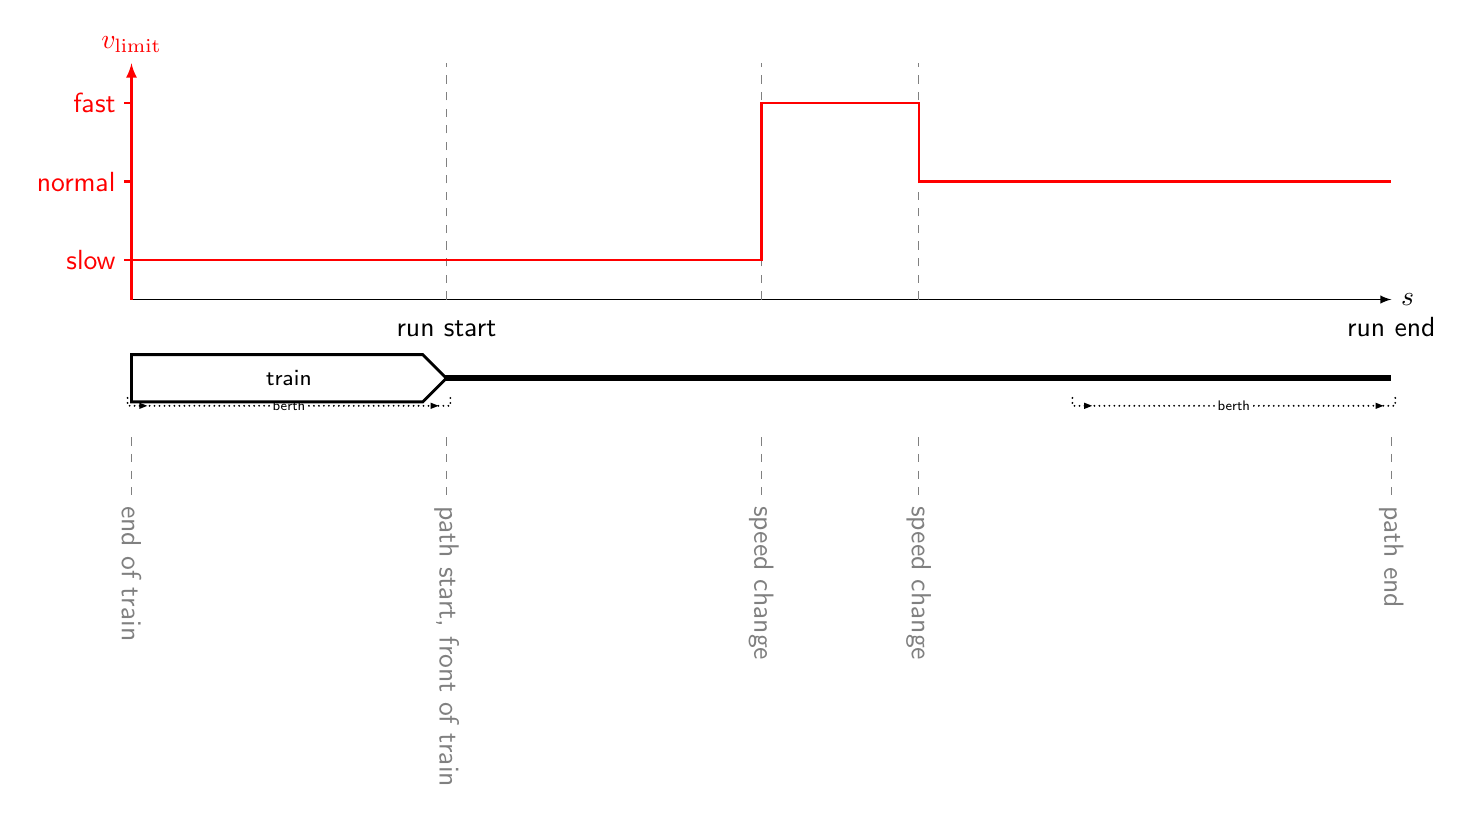
\begin{tikzpicture}[font=\sffamily]
  \usetikzlibrary{calc}
  \tikzset{
    label/.style={anchor=base,above=0.4cm},
    helper/.style={foreground!50!background,dashed},
    speed/.style={thick,red},
  }

  % A: end of train (length 4cm) = origin of v_limit axis
  % B: path start = front of train = run start
  % C, D: speed changes
  % E: run-end berth
  % F: path end = run end
  \coordinate (A) at (0,0);
  \coordinate (A1) at (2,0);
  \coordinate (B) at (4,0);
  \coordinate (C) at (8,0);
  \coordinate (D) at (10,0);
  \coordinate (E) at (14,0);
  \coordinate (F) at (16,0);

  \coordinate (hb) at (0,-1.5);

  % axis
  \draw[->,>=latex]          ([shift={(0,1)}] A)                        -- ([shift={(0,1)}] F) node[right] {$s$};
  \draw[->,>=latex,speed]    ([shift={(0,1)}] A)                        -- ++(0,3) node[above] {$v_\mathrm{limit}$};
  \draw[shorten <=3pt,speed] ([shift={(-0.2,1.5)}] A) coordinate (v80)  -- ++( 0.2 , 0) node[left=0.2em] {slow};
  \draw[shorten <=3pt,speed] ([shift={(-0.2,2.5)}] A) coordinate (v120) -- ++( 0.2 , 0) node[left=0.2em] {normal};
  \draw[shorten <=3pt,speed] ([shift={(-0.2,3.5)}] A) coordinate (v160) -- ++( 0.2 , 0) node[left=0.2em] {fast};

  \draw[helper]    ([shift={(0,1)}] B) -- ++(0,3);
  \draw[helper]    ([shift={(0,1)}] C) -- ++(0,3);
  \draw[helper]    ([shift={(0,1)}] D) -- ++(0,3);

  % speed limit
  \draw[speed]
    let  \p{A}=(A), \p{C}=(C), \p{D}=(D), \p{F}=(F),
        \p{8}=(v80), \p{12}=(v120), \p{16}=(v160)
    in (\x{A},\y{8}) -- (\x{C},\y{8}) -- (\x{C},\y{16}) -- (\x{D},\y{16}) -- (\x{D},\y{12}) -- (\x{F},\y{12});

  % track schematic
  \maintrack (A) -- (F);

  \berth[forward] at (A1) length (berth);
  \train[forward] at (B) label (train);
  \node[label] at (B) {run start};

  \berth[forward] at (E) length (berth);
  \node[label] at (F) {run end};

  \tikzset{hectometer base={(hb)},orientation=right}
  \hectometer[] at (A) mileage (end of train);
  \hectometer[] at (B) mileage (path start, front of train);
  \hectometer[] at (C) mileage (speed change);
  \hectometer[] at (D) mileage (speed change);
  \hectometer[] at (F) mileage (path end);
\end{tikzpicture}\end{document}
